\item {\bf Exponentially-Weighted Averager} An exponentially-weighted averager
  that produces an output signal that is a weighted sum of a series of input
  signals described by:

  \begin{center}
$S_{o} = \frac{1}{m}\left[S_n + \left(\frac{m-1}{m}\right)S_{n-1}+\left(\frac{m-1}{m}\right)^2S_{n-2} + \ldots\right],$
  \end{center}
  
where $m$ is the exponential weighting factor.
  
\begin{enumerate}
    \item Demonstrate how $m$ affects the weighting of more recent or later samples in the exponential averager.  You can do this numerically, and not analytically.
    %\item We derived the SNR improvement associated with an equally-weighted and boxcar averager to be $\sqrt{N}$, where $N$ is the number of samples being averaged.  Derive the SNR improvement for the exponentially-weighted averager (hint - it should be a function of $m$). [1 point]
    \item We discussed in lecture how the boxcar averager acted as a low-pass
        filter on the data.  Sketch the transfer function of the boxcar
        averager relative to a sinusoidal signal oscillating at $\omega_o$, and
        demonstrate how if the averaging window is too long, then you are just
        left with the DC offset of the sinusoidal signal in the output. 

    \item Compare and contrast the frequency-domain transfer function of a
        boxcar averager with that of an exponentially-weighted averager.  How
        does the transfer function of the exponentially-weighted averager
        change as a function of $m$?
\end{enumerate}


$$S_{o} = \frac{1}{m}\left[S_n + \left(\frac{m-1}{m}\right)S_{n-1}+\left(\frac{m-1}{m}\right)^2S_{n-2} + ...\right]$$

Lets see how the weights change as a function of $m$ for 30 samples (Figure~\ref{fig:exp_weight_ave}).

\begin{figure}[htb!]
\centering
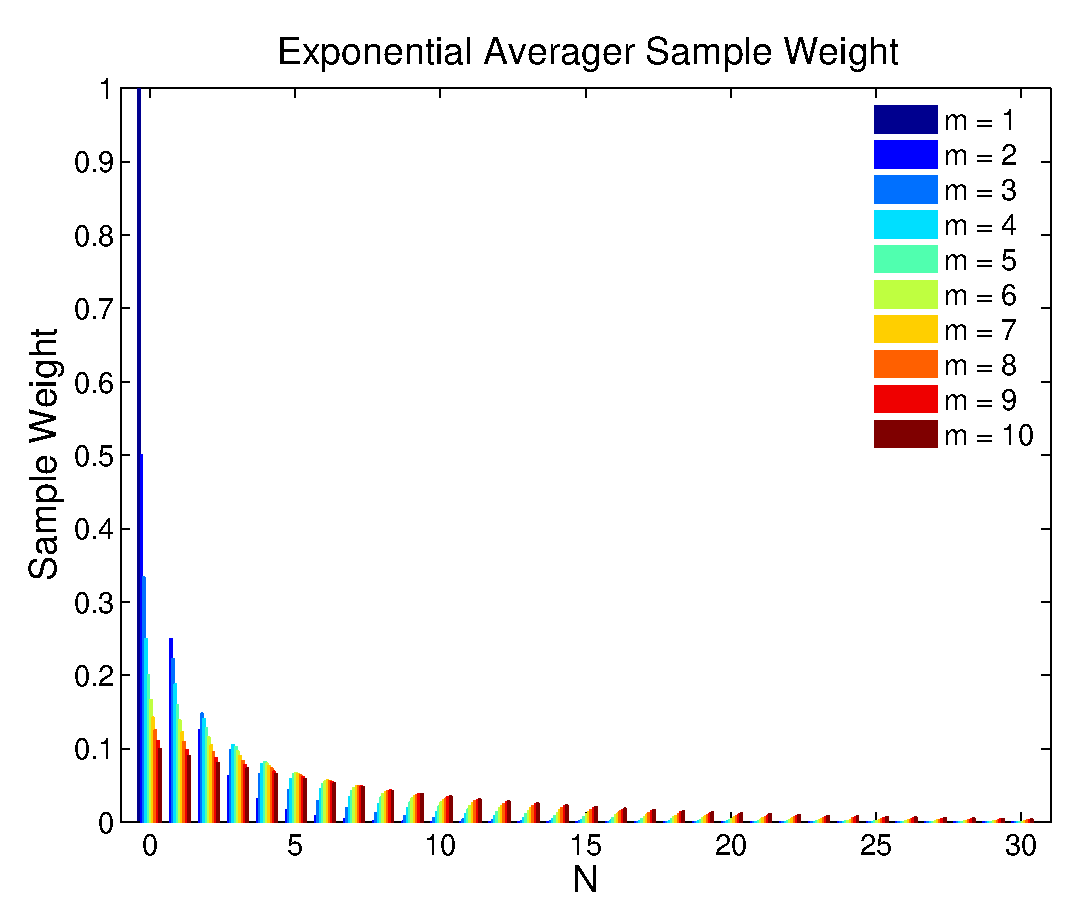
\includegraphics[width=0.5\linewidth]{exp_weight_averager/exp_weight_ave.eps}
\caption{Weights for samples in an exponential averager as a function of $m$.}
\label{fig:exp_weight_ave}
\end{figure}

Notice that as $m$ increases, the impact of older samples increases.  In the
limiting case ($m$ = 1), we simply have a delta function for the most recent
sample.  Question to consider: How does the overall energy of the output signal
change as a function of $m$?  Is it constant?

The SNR improvement of the exponential averager is a function of $m$.  There is no SNR improvement for $m = 1$.

For the exponential averager, the new average estimate ($A_m$) can be related to the previous estimate ($A_{m-1}$) with a new input ($I_m$), as:

\begin{equation}
A_m = A_{m-1} + \frac{I_m - A_{m-1}}{m} = \frac{1}{M}\displaystyle\sum_{i=1}^m \left( \frac{M-1}{M}\right)^{m-i} I_i,
\label{eqn:expSNR}
\end{equation}

where $M$ is the number of samples with history in the averager.

The derivation of the SNR associated with the exponential averager can be expressed after expansion of Equation~\ref{eqn:expSNR} as:

\begin{equation}
\displaystyle\lim_{m \rightarrow \infty} \textrm{SNR}_\textrm{o} \frac{\left[ 1-(1-\frac{1}{M})^m \right]}{\left[ \frac{1-(1-\frac{1}{M})^{2m}}{2M-1}\right]^{\frac{1}{2}}} = \textrm{SNR}_\textrm{o} (2M-1)^{\frac{1}{2}},
\end{equation}

where $\textrm{SNR}_\textrm{o}$ is the original signal SNR.

The filtering characteristics of the boxcar averager, as a function of the length of the boxcar, are shown in Figure~\ref{fig:boxcar_fft}.  Notice how for a single sample boxcar length (i.e., a delta function), all frequencies are passed (i.e., a uniform transfer function), but as the length of the boxcar increases, the passband of the transfer function reduces down to something that, in the extreme, would be a delta function at $f$ = 0, only allowing DC characteristics to be preserved.

\begin{figure}[htb!]
\centering
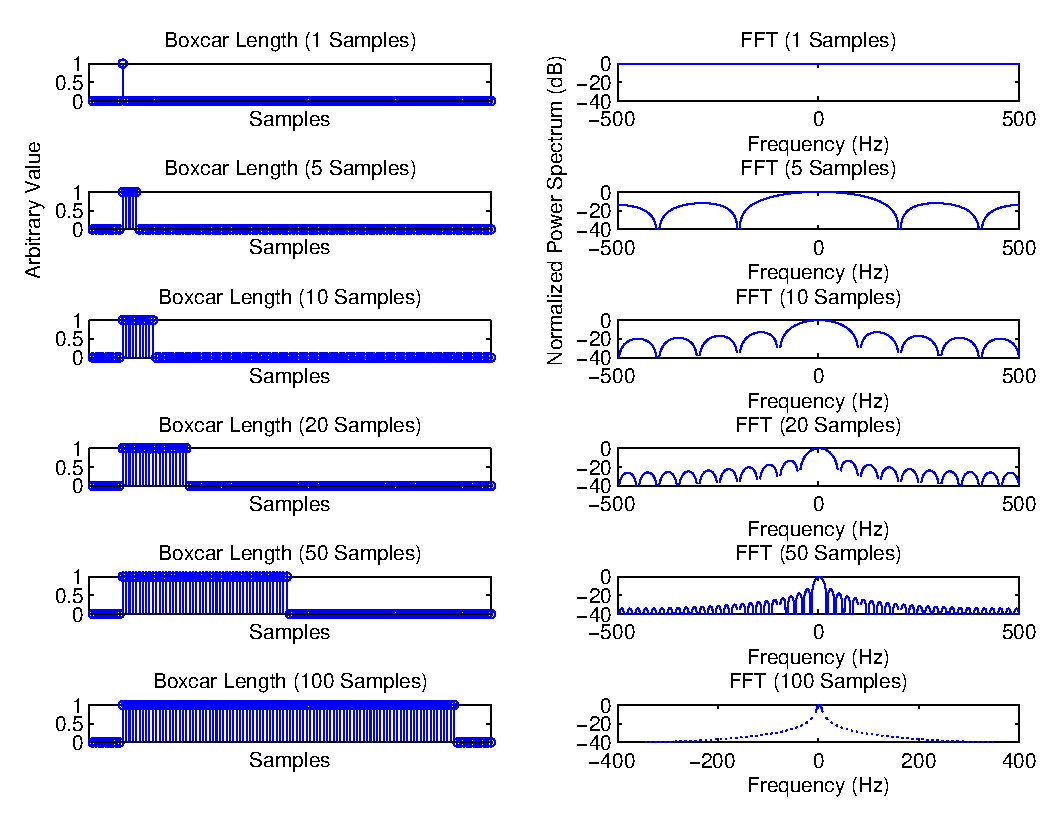
\includegraphics[width=1.0\linewidth]{boxcar_averager/boxcar_fft.eps}
\caption{Magnitude transfer functions for different length boxcar averagers.  The sampling frequency was arbitrarily set to 1 kHz.}
\label{fig:boxcar_fft}
\end{figure}

To compare/contrast, the power spectra of the exponential averager for 3 different $m$ weights are shown in Figure~\ref{fig:exp_fft}.  Notice how for increasing $m$, the passband of the exponential averager transfer function becomes significantly limited, effectively acting as a low-pass filter, similar to what happens with the boxcar averager, but to less of an extreme.

\begin{figure}[htb!]
\centering
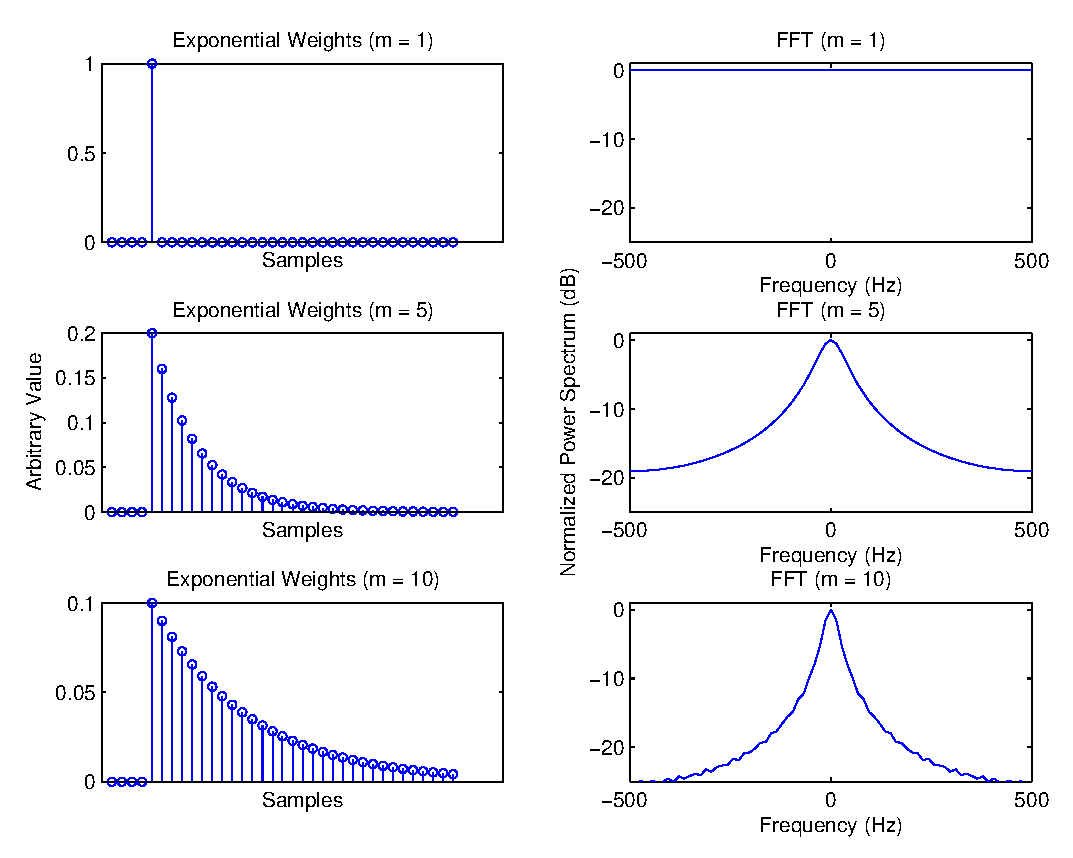
\includegraphics[width=1.0\linewidth]{exp_weight_averager/exp_weight_ave_fft.eps}
\caption{Magnitude transfer functions for differently weighted exponential averagers .  The sampling frequency was arbitrarily set to 1 kHz.}
\label{fig:exp_fft}
\end{figure}

Code for various plots shown in these solutions is as follows:

\verbatiminput{boxcar_averager/sliding_average.m}
\verbatiminput{boxcar_averager/boxcar_fft.m}
\verbatiminput{exp_weight_averager/exp_weight_ave.m}

